
%   dvips -O 2mm,-9mm -T 215mm,280mm 模版.dvi        %成品
%   E:\2015年\电子学报-杂志\原稿\模板 2015.7.21

%   dvips -O -13mm,-25mm -T 190mm,260mm 模版.dvi      打样

%\documentclass[twoside,draft]{article}  %\陈清华改
\documentclass[twoside]{article}
\usepackage{multicol,headrule,ams2la}
\usepackage{graphics}
\usepackage{bm}     % 英文黑斜体
\usepackage{xcolor}
\usepackage{amssymb}                  % 数学字体、符号
\usepackage{amsbsy} %公式中黑斜体

\usepackage{graphicx,subfigure} 
\usepackage{multirow}
%用法$ \boldsymbol{XX}$ 也可自定义简单用法, 见下面自定义的\pmb
\graphicspath{{figs/}}      %定义图的存放路径
%------------------------ Page Format --------------------------
\columnsep=0.5cm \columnseprule=0pt \footskip=6truemm \headsep 0.2
true cm \textheight 24.0 true cm \textwidth 18 true cm
%\parindent 1 true cm
\topmargin =-3mm
\oddsidemargin = -0.9cm %1.6 true cm
\evensidemargin = -0.9cm %1.6 true cm

\def\le{\leq}
\def\ge{\geq}
%\def\leq{\leqslant}
%\def\geq{\geqslant}
\def\zd{{\rm d}}
\def\zT{{\rm T}}
\def\zth{{\rm th}}
\def\znormal{{\rm normal}}
\def\ds{\displaystyle}
\def\dl{\displaystyle}
\newcommand{\inlinedComment}[2]%{}% EMPTY for submission
	{\textcolor{#1}{\small\textit{#2}}}
\newcommand{\ksc}[1]{\inlinedComment{red}{SC says: #1}}
\newcommand{\zfl}[1]{\inlinedComment{blue}{FL says: #1}}

\graphicspath{{figs/}}      %定义图的存放路径

\setcounter{page}{1} \nofiles
\renewcommand{\baselinestretch}{1.06}
%上一行是定义正文行距的, 现在是单倍, 把1.06改成1.4或更大, 行距就加大, 成隔行
\renewcommand{\arraystretch}{1.03}
%上一行是定义表格行距的, 也可加大
%%%%%%%%%%%%%%%%%%%%%%%%%%%%%%%%%%%%%%%%%%%%%%%%%%%%%%%%%%%%%%%%%
\def\oddhead{{\rm\hfill\protect\small
The Latex Template of CJE %     单页书眉, 填入论文标题即可, 请尽量把书眉控制在12cm内
\hfill }}
\def\evenhead{{\rm \hfill \protect\small\it Chinese Journal of
Electronics  \rm\hfill 2016}}
\def\sub#1{\par\vskip1.5\baselineskip\par\centerline{\large\bf
#1}\par\vskip0.5\baselineskip\par}
%标题行可用\sub{}
\def\RE{\par\vskip1.5\kh\par\centerline{\bf
References}\par\vskip0.5\kh\par}
\def\REF#1{\par\hangindent\parindent\indent\llap{#1\enspace}\ignorespaces}
%参考文献可用\REF{[1]}
\DeclareSymbolFont{lettersA}{U}{txmia}{m}{it}
\DeclareMathSymbol{\piup}{\mathord}{lettersA}{25}
\DeclareMathSymbol{\muup}{\mathord}{lettersA}{22}

%%%%%%%%%%%%%%%%%%%%%%%%%%%%%%%%%%%%%%%%%%%%%%%%%%%%%%%%%%%%%%%%%%%
\begin{document}
\newtheorem{theorem}{Theorem}
\newtheorem{proposition}{Proposition}
\newtheorem{remark}{Remark}
\newtheorem{proof}{Proof}
\def\footnoterule{\kern 1mm \hrule width 12cm \kern 2mm}
\abovedisplayskip=8.0pt plus 2.0pt minus 1.5pt
\belowdisplayskip=8.0pt plus 2.0pt minus 1.5pt
 \def\thefootnote{}
\TagsOnRight
\def\kh{\baselineskip}
%\def\pmb#1{\boldsymbol{#1}}

%====================================================================
\thispagestyle{empty}
%************************************************************************
\noindent Chinese Journal of Electronics

\noindent Vol.25, No.1, Jan.\ 2016

\vskip 2cm

\begin{center}\huge\bf
%这行放入论文标题
Machine-Learning Aided Analysis of Clone Evolution$^*$
\end{center}\footnotetext{\footnotesize {Manuscript Received xx xx, xxxx; Accepted xx xx, xxxx.}\ This work is supported
by the National Natural Science Foundation of China (No.xxxxxxxx).
%这行放入收、修稿日期及基金资助
}

\vskip 4mm

\begin{center}\large\rm
XXX XXX$^{1}$, XXX XXX$^{2}$ and XXX XXX %这行放入作者姓名
\\\vskip1mm
{\small(1.~\it XXXX, XXXX, XXXX, XXXX%这行放入作者单位2
\rm)}

{\small(2.~\it XXXX, XXXX, XXXX, XXXX%这行放入作者单位2
\rm)}

\footnotetext{\footnotesize \copyright~2016 Chinese Institute
of Electronics. DOI:10.1049/cje.2016.0X.0XX}
\end{center}

\begin{multicols}{2}%双栏开始

{\footnotesize\bf Abstract --- {\footnotesize\bf
%这里放Abstract
Code clones are similar code fragments appearing in software. As software evolves, code clones may be subjected to changes as well; we term this clone evolution. %Researchers have proposed several methods to detect clones and their associated clone groups, and used clone genealogy and clone patterns to describe their evolution. 
There have not been many investigations into characteristics of clone evolution. In this paper, we tackle this question by exploring useful information associated with changes of clones during evolution. We focus on three perspectives of clone evolution, ranging from individual clone changes to characterization of clone genealogies. We identify metrics that capture clone changes. With the help of a machine-learning technique called X-means clustering, we establish associations between clone changes and life times of clones. We conducted experiments on the repositories of two open source softwares, {\em ArgoUML} and {\em jEdit}.  Our results show that clones are mostly stable (without any changes) throughout software evolution. For the relatively smaller group of ``unstable'' clones, changes to clones usually happen after several versions of software evolution, and consistent changes (to clone groups) appear more frequently than inconsistent ones. We therefore suggest that developers should pay more attention to clones in relatively longer genealogies, and should consider applying changes consistently to all clones within a clone group when a constituent clone fragment has undergone change. %We believe that these characteristics of clone evolution are helpful for developers to understand and maintain the clones.
}

\bf Key words --- {\footnotesize\bf
Code clones; Clone analysis; Clone characteristic;  Clone metrics; Machine learning.}}


%\begin{center}{\large\bf I.\ Introduction}\end{center}
%\begin{center}{\large\bf I.\ Introduction}\end{center}
\begin{center}{\large\bf 1.\ Introduction}\end{center}

Code clones are collection of code fragments which are similar to one another according to some definition of ``similarity''[1]. They may take up 7-23\% of the software, even 59\% in some software[2]. %Clones are often the result of copy-and-paste activities, and there are several other factors for their existence, such as adoption of reuse approach, programming approach, and maintenance benefits. 
%Researchers propose several methods to detect clones, such as NiCad. which can be divided into Text-based, Token-based, AST-based, PDG-based and others according to their technology. With appropriate clone detection tools (such as NiCad), we can detect clones within a software.  
As clones always evolve with the softwares, Kim et al. propose clone genealogies to describe this evolution process, and provide several clone patterns to categorize different clone change during their evolution[3]. This has led to a new research direction focusing on clone evolution and clone patterns. Currently, there are tools available for detecting clones and building clone genealogies. Their availability has led to numerous work on clone analyses, such as studies on clone stability and clone patterns [5,6]. %This can guide developers to understand the clones. 

At the same time, there has been contraversial debates over the usefulness of clones in software. Some researchers opine that the presence of clones is harmful, as they can incur additional maintenance effort [4], and even cause software defects. For instance, clones that change inconsistently during software evolution are likely to lead to defects [5]. Consequently, developers should take measures to avoid clone creation, remove clones through refactoring. Other researchers take a positive outlook towards the existence of clones. They view code clones as mainly a by-product of reuse, and most of the clones created turn out to be more stable than non-clones, and thus can save much development time [6]. 

%A good understanding of clones and their evolution can provide strong assistance to software maintenance.  
Regardless of different opinions, clones can naturally be found in software, as ``copy-and-paste" way of producing code (and thus creating clones) remains efficient in software development. It is therefore important to understand clone characteristics and how they impact development and maintenance in software evolution. Such investigation result can have substantive help on clone anlaysis and management.    Specifically, 
We are interested in deriving relationships; we name these relationships {\em clone evolutionary characteristic}. 
They can offer fresh insight from the evolutionary aspect of clones in a piece of software. Throughout the paper, we use the terms ``clone evolutionary characteristics'', ``clone characteristics'' and ``characteristics'' interchangeably.  

%We consider three different perspectives from three different clone entities: clone fragment, clone group and clone genealogy. Clone fragment offers an individual perspective about clones. It tells us how individual clones are changed during evolution. Clone group offers a regional perspective about clones. %It shows us how a group of similar clones is being operated upon during evolution. Clone genealogy offers a global perspective about clones. %It tells us how clone groups are evolved from beginning till the end of our investigations.

In this paper, we propose an approach to explore and analyze clone characteristics through a machine learning method. We build clone genealogies through mapping clones between neighboring versions. After that, we extract several metrics at three levels to represent three different clone entities: {\em Clone Fragment, Clone Group and Clone Genealogy}. These metrics can cover many interesting and relevant information about clone entities. Lastly, we use  X-means clustering implemented by WEKA (short for ``Waikato Environment for Knowledge Analysis''[25]) to cluster all the clones.
We conduct an empirical study on two open-source software packages. 

Our study 
shows that clones are in general very stable during their evolution, and clones usually do not undergo changes at the infancy stage of evolution. Developers should therefore pay more attention to (more matured) clones that have existed in a genealogy after several evolutions (aka., in longer life clone genealogy). We also suggest that developers should consider the possibility of making consistent changes across the entire clone group when one of the constituent clone fragments has undergone change.  The contributions of this paper are as follows:
\begin{enumerate}
\setlength{\itemsep}{0pt}
\setlength{\parsep}{0pt}
\setlength{\parskip}{0pt}
\item  We propose a framework to analyze the clones to explore clone evolutionary characteristics, which are meaningful to clone analysis and maintenance.
\item We view clones as one kind of data from three different perspectives: clone fragment, clone group and clone genealogy, and extract some metrics to present the clones respectively.
\item  We conducted an empirical study on two open source software, and obtain interesting findings which can give developers some suggestions to better understanding and maintaining clones in particular, and software in general.
\end{enumerate}

Our paper is organizing as follows. Section 2 is the related work. %We give a brief introduction of clone research. %Section 3 is our motivation. We explain why we want to do this work. We explain the clone evolution characteristic of clones. 
Section 3 is our method which explain how to analyses the clones. %Details can be seen in the following parts in this paper. 
Section 4 is our case study. %We give the experiment systems, and the steps we take in the experiment. 
Section 5 is our analysis and results. %We analyze the results about clone characteristic. 
Section 6 is discussion. Section 7 is our conclusion. 

%\begin{center}{\large\bf III.\ Motivation}\end{center}

%With appropriate clone detection tools (such as NiCad), we can detect clones within a software. Clones are enveloping with software. Clone genealogies can describe clone evolution from successive versions of software, and clone patterns can describe clone change during their evolution. We believe that there should be some relationship in clones and their evolution. However, how to analyze these clones and their evolution to find the relationships, which can help developers understand clones? In our earlier work, we clustered clone fragments to find relationships between clone lifes and clone patterns, and derive that the short-life clone fragment may be more frequently changed than the long-life ones. We believe more can be derived/inferred from a good collection of information extracted from clone groups and their genealogy. Specifically, we are interested in deriving relationships between clones and their evolution; we name these relationships {\em clone evolutionary characteristic}.

%Clone evolutionary characteristic is the clone relationships between the clones and their evolution, which can help developers to understand and maintain the clones. Clone evolutionary characteristics adds new values to existing clone analysis and maintenance tasks, as it offers fresh insight from the evolutionary aspect of clones in a piece of software. Throughout the paper, we use the terms ``clone evolutionary characteristics'', ``clone characteristics'' and ``characteristics'' interchangeably. 

%In order to explore more clone characteristics from clones and evolution, we consider three different perspectives from three different clone entities: clone fragment, clone group and clone genealogy. A clone fragment offers an individual perspective about clones. It tells us how individual clones are changed during evolution. Clone groups offer a regional perspective about clones. It shows us how a group of similar clones is being operated upon during evolution. Lastly, a clone genealogy offers a global perspective about clones. It tells us how clone groups are evolved from beginning till the end of our investigations. 

%In this work, we adopt a machine-learning algorithm named X-means to the discovery of clone evolution characteristics. We shall describe this approach in detail in the following section.


%\begin{center}{\large\bf II.\ Related Work}\end{center}
\begin{center}{\large\bf 2.\ Related Work}\end{center}

%In recent years, clone research community has increasingly turned its attention to clone management. In general, clone management can be divided into three parts: clone detection, clone analysis and clone maintenance [7,8]. Functionally, clone detection discovers clones in software; clone analysis assists developers in understanding clones, and clone maintenance aims to solve issues arisen from the presence of clones, as well as to make full use of their presence.  

The most popular activity on clones is clone detection. In past decades, researchers have proposed several methods to detect clones, and rolled out a number of effective clone detection tools, such as NiCad [9], CCFinder [10], etc. %According to the technology deployed, these clone detection methods can be classified into different bases: Text, Token, AST, PDG and Metrics. %NiCad is a clone detection method that has been shown to yield both high precision and high recall in near-miss intentional clones. CCFinder can effectively detect clones based on token, and also can effectively identify specific characteristics of software. 
Interested readers can refer to [17] for a detailed review of clone detection based on a comprehensive set of 213 articles. Unfortunately, clone detection alone does not significantly mitigate software maintenance cost. Therefore, clone management issues become increasingly popular in this research community [7,8]. %The most popular clone management activity is clone refactoring. Researchers propose several methods to identify refactoring opportunities and to refactor clones. At the same time, several clone management tools have been built.
JSync [12], a novel clone management tool, which can help developers to manage clone evolution relation and inconsistent change. CloneTracker [18], an Eclipse plug-in, provides support for tracking code clones in evolving software. CeDAR [11], also an Eclipse plug-in, can forward clone detection results to the refactoring engine in Eclipse. 

There is also a significant amount of attention on {\em clone analysis}%., such as clone classification, clone evolution, and clone evaluation. As clone analysis 
, which improves the understanding of clone development and clone impact on software. %, it has been an important research activity since a decade ago. 
Jiachen Yang proposes a classification model that applies machine learning on the judgments made by individual users regarding code clones [15]. Wei Qu proposes a novel pattern mining framework for cloned codes in software systems [16]. % It efficiently exploits software's spatial information as well as graph information and thus can mine accurate patterns of cloned codes for software systems.  
Yun Lin presents an approach to automatically detect differences across multiple clones[24].%; they also have implemented an Eclipse plugin and evaluated its accuracy with respect to three Java software systems .

Code clones evolve with software, and researchers maintain a strong interest in the patterns in which clone changes through software evolution. Kim et al. propose the concept of {\em clone genealogy} to describe evolution, and notice that clone refactoring may not always improve software quality [3]. % because of the following reasons: either a clone may be short lived, or a long-living clone which has changed consistently is usually not easily refactorable. 
Duala-Ekoko proposes a clone tracking system, which produces Clone Region Description for tracking clone evolution, and notifies clone modifications to developers [19]. Bakota presents an approach for mapping code duplications% from one particular version of software to another one. He 
, and proposes a definition of clone smell, which help developers determine clones which show signs related to software defects [20, 21]. Krinke finds that clone code is more stable than non-cloned code, and also older than non-cloned code on average [6]. Bettenburg observes that %only 1.02\%-4.00\% of all clone genealogies introduce software defects at the release level, and suggests that 
clones do not have significant impact on the post-release quality of the studied softwares [13]. Harder finds that clone stability depends on clones' characteristics corresponding to the project environment [22].

There is continuing debate on clone harmfulness. The proponent for clones being harmful holds the view that %the existence of clones can incur additional maintenance effort, and 
clones inconsistently changed during software evolution may lead to software defects[5]. The opponent holds that clones are in general more stable than non-clones during software evolution [6]. Foyzur Rahman %analyzes the relationship between clone and defect proneness. He 
finds that, firstly, a great majority of bugs are not significantly associated with clones. Secondly, clones are less defect prone than non-cloned code [23]. There are also others who adopt a neutral attitude towards the harmfulness of clones. Cory Kapser describes several patterns of clone, and discusses their pros and cons [4]. Some researchers apply Bayesian Networks, a machine-learning technique, to predict the harmfulness of an intended code cloning operation[14]. We take the view, and as shown in the finding in this work, that clones' existence is by nature of the habits taken by developers during software development, and attention paid to consistency in changes in clones during evolution can pay off in mitigating software maintenance effort. 



%\begin{center}{\large\bf III.\ Methodology}\end{center}
\begin{center}{\large\bf 3.\ Methodology}\end{center}

\leftline{{\bf 3.1 \ The Framework of clone characteristic analysis}}

Fig.1 is the framework of our clone characteristic analysis with machine learning, which can be divided into:  pre-processing, metric extraction and characteristic analysis. During pre-processing, we build the corresponding clone genecology by linking and relating groups of clones across consecutive versions of the software. At metric extraction, we identify and extract a set of metrics to represent clone fragments, clone groups and clone genealogies respectively. These metrics capture the relevant information about the clones and their evolution. Finally, in characteristic analysis stage, we use machine learning technique to explore the clone evolutionary characteristics from clones and their evolution.

 \vskip 2mm
\centerline{\includegraphics[width=3.3in]{Fig1} }
\vskip 1mm
\centerline{\footnotesize\begin{tabular}{c} Fig.\ 1.\  The Framework of Clone Characteristic Analysis
\end{tabular}}
\vskip 0.5\baselineskip%插图结束

\leftline{{\bf3.2 \ Pre-processing }}

In this stage, we aim to build clone genealogies according to the detected clones from consecutive versions software.  We firstly obtain consecutive versions of open source software, % from websites and the version control system subversion, 
and detect all clones in each software version with NiCad. %, which produces grouped clones by their similarity.
After that, we use %CRD to describe clones, and 
build clone genealogies by associating neighboring clone fragments and clone groups. 

{\em Clone detection with NiCad and Representation using CRD (Clone Region Descriptors)}. NiCad % is a clone detection tool, which 
can find identical clones and near-miss clones efficiently. We use the default configuration to detect all clones from each software version. %It detects clones with two different granularities: functions and blocks. Because {\em block level} is more general (function clones are part of block clones), we use the default configuration of {\em block level} to detect all clones from each software version. The results are kept in XML files, which mark clone fragments with {\em ``Filename + Line No''}, 
This can group all clone fragments into various clone groups. %, according to their similarity. 
In order to build clone genealogies, we use a modified version of CRD to describe clone fragments, which is proposed by Duala-Ekoko. 
A CRD is an abstract description of clone location, which includes the file name, method name, and combines syntactic, structural and lexical information [19]. %We improve CRD with our purpose. 
We combine CRD, {\em LocationOverlapping} and {\em TextSimilarity} to relate clones in two neighboring versions.   {\em LocationOverlapping} can help to locate the clone in source code [3], and computes an overlapping score between a location of clone fragments in version $i$ and version $i+1$. {\em TextSimilarity} can be used for comparing the similarity of clone fragments, which is defined in NiCad [9]. It computes the percentage of common code lines for two clone fragments. 

%We improve the CRD prototype for our purpose, which are defined in previous work [27].

{\em Mapping clone group and building clone genealogy}. %In order to build a clone genealogy, 
We map all the clone fragments and clone groups between two consecutive versions. %The mapping algorithm is called CRD-based Clone Group Mapping Algorithm. 
Given two adjacent versions {\em $v_i$} and {\em $v_{i+1}$}, we compare (using CRD, as desribed earlier) each clone fragment in {\em $v_i$} against each clone fragment in {\em $v_{i+1}$}, and produces pairs of mapping clone fragments, such that for each pair, (1) the first clone fragment comes from {\em $v_i$} and the second {\em $v_{i+1}$}, and (2) the clone groups  can also be mapped with matching clone fragments. %The details of the algorithm are described in our previous work [25]. 
Next, we can build clone genealogies for the software based on the mapping clone groups.  %After clone group mapping, w

We can describe clone group changes during its evolution as {\em ``clone pattern''}. More formally, each clone group (called CG) can contain several clone fragments (called CFs). Consider a clone group that exists in two neighboring versions. Let {\em srcCG} denote the clone group in the former version, and {\em destCG} denote the clone group in the latter version. Changes from {\em srcCG} to {\em destCG} are described by clone patterns, and they become the metrics associated with {\em destCG}. %(and not {\em srcCG}). 
The clone patterns are defined by Kim[3], which are given as follows: %Interested readers can refer to [25] for details.  
\begin{itemize}
\setlength{\itemsep}{0pt}
\setlength{\parsep}{0pt}
\setlength{\parskip}{0pt}
\item {Static}: no change in clone fragment  (number and content).
\item {Same}: no change in number of clone fragment, but the  content of fragment may change.
\item {Add}: number of clone fragment increases.
\item {Subtract}: number of clone fragment decreases.
\item {Consistent Change}:  all clone fragments change consistently.
\item {Inconsistent Change}: clone fragments change inconsistently.
\item {Split}: inconsistent change beyond a threshold, causing the clone group to split into two clone groups.
\end{itemize}

Fig.2 gives an example of clone genealogy and clone patterns. In this example, the clone genealogy is constructed from 5 versions of the software. 
From version {\em i} to {\em i+1}, the clone group is enlarged with two new clone fragments, so its associated clone pattern is {\em add}. In the next version change, the clone group is split into two groups, which have different clone patterns (one is {\em subtract}, and the other is {\em consistent change}). From version {\em i+2} to {\em i+3}, clone patterns are {\em sub} and {\em inconsistent change} respectively. In the last version, clone patterns are {\em add} and {\em sub} respectively.

 \vskip 2mm
\centerline{\includegraphics[width=3.0in]{Fig2} }
\vskip 1mm
\centerline{\footnotesize\begin{tabular}{c} Fig.\ 2.\  An Example of Clone Genealogy[3]% \\ Capturing the Evolution of Code Clones 
\end{tabular}}
\vskip 0.5\baselineskip%插图结束

\leftline{{\bf3.3 \ Clone Metrics}}

As typically done in machine learning, we represent a clone by a vector of features, which are called {\em clone metrics}. These features are extracted from clone fragments, clone groups and clone genealogies. 

{\em The metrics for clone fragment}. A clone fragment gives an {\em individual} perspective of clones. %, which are code fragments in software. 
During its life, the fragment can be modified by the developer, especially during software maintenance. %Further, clone fragment can change drastically. 
Thus, we consider as metrics the number of times the clone changes and the change made from last version. Therefore, the metrics for clone fragment in version $i$ are as follow:

\begin{itemize}
\setlength{\itemsep}{0pt}
\setlength{\parsep}{0pt}
\setlength{\parskip}{0pt}
\item {Clone Life}: number of versions which the clone fragment exists in software so far (until version i).
\item {Ischanged}:	equals 1 if the Clone fragment in version i is changed from the last version (version i-1); 0 otherwise.
\item {Change Times}:	number of times the clone fragment changed so far (up till version i) in the evolution.  
\end{itemize}

{\em The metrics for clone group}. Clone group offers a {\em regional} perspective of clones, where the region is defined by the group. %Here, clones from one version of software are organized into clone groups.
For a clone group% found in a version of the software
, it is important to capture the length of its life so far. %During evolution, a 
Clone group may change from last version to the current version. This change is called {\em clone pattern}, %Clone patterns for the group 
which can give us a change summary throughout evolution. We therefore extract life and clone patterns as clone group  in version $i$ metrics as follow:

\begin{itemize}
\setlength{\itemsep}{0pt}
\setlength{\parsep}{0pt}
\setlength{\parskip}{0pt}
\item {Group Life}: number of versions which clone group exists in software till version $i$.
\item {Static}:	all clone fragments in group are static from last version.
\item {Same}:	clone group undergoes a ``same'' pattern change from  last version.
\item {Add}: clone group undergoes an ``add'' pattern change from last version.
\item {Subtract}: clone group undergoes a ``subtract'' pattern change from last version.
\item {Consistent Change}: clone group undergoes a ``consistent change'' pattern from last version.
\item {Inconsistent Change}: clone group undergoes an ``inconsistent change'' pattern from last version.
\item {Split}: clone group undergoes a ``split'' pattern change from last version.
\end{itemize}

{\em The metrics for clone genealogy}. Clone genealogy provides a {\em global} perspective of the clones, capturing the entire clone evolution occurring in all versions. %There are lots of clone genealogies in a piece of software. 
%We extract the {\em genealogy life} and the {\em number of clone patterns} to represent clone genealogy. 
{\em Genealogy life} is an important metric for clone genealogy.
As clone genealogy describes how this clone group changed(clone pattern) throughout its life,  %As these changes can tell us about the genealogy change history, 
we capture the {\em genealogy life} and the {\em number of clone patterns} which clone genealogy had experienced in its whole life. Therefore, the metrics include the following:
\begin{itemize}
\setlength{\itemsep}{0pt}
\setlength{\parsep}{0pt}
\setlength{\parskip}{0pt}
\item Genealogy  Life: number of versions which clone genealogy exists in software.
\item Static Number: number of ``static'' pattern which all clone groups belonging to this genealogy have experienced in its life.
\item Same Number: number of ``same'' pattern which all clone groups belonging to this genealogy have experienced in its life.
\item Add Number: number of ``add'' pattern which all clone groups belonging to this genealogy have experienced  in its life.
\item Subtract Number: number of ``subtract'' pattern which all clone groups belonging to this genealogy have experienced in its life.
\item Consistent Number: number of ``consistent pattern'' which all clone groups belonging to this genealogy have experienced in its life.
\item Inconsistent Number: number of ``inconsistent pattern'' which all clone groups belonging to this clone genealogy have experienced in its life.
\item Split Number: number of ``split'' pattern which all clone groups belonging to this genealogy have experienced in its life.
\end{itemize}

\leftline{{\bf3.4 \ Clone Characteristics Mining}}

In order to mine clone characteristics, %from the clones and their evolution, we use WEKA to analyze the clone entities, which are: clone fragments, clone groups and clone genealogies. 
we divide this mining task into two subtasks. First, we obtain the statistics about the occurrences of metrics in each of these clone entities, and investigate the characteristics of these clone entities. Second, we use WEKA to cluster these clone entities. In this subtask, our main goal is to characterize the timing aspects of clone changes during software evolution. Specifically, we aim to determine the time during evolution when clone changes begin to take place. %To this end, we employ tools in WEKA to perform clustering of clone entities that include time elements. 

Employing WEKA for this task involves two parts: First, we generate a vector named ``clone vector'' with all the metrics (including timing metrics) for each clone entity. Second, we use WEKA to cluster these vectors, and investigate the results obtained from clustering. %Let's elaborate further. 

 {\em Generating clone vectors}. For each clone fragment, group and genealogy, its vector is an $m$ dimensional vector: {$V$= {($v_1$, $v_2$, $...$, $v_m$)}}, where $v_i$ features a specific metric mentioned in the previous subsection. When we generate vectors for all clones, we obtain a clustering vector space X for all clones, which can be defined by {$X$= {($x_1$, $ x_2$, $...$, $ x_n$)}}, where $n$ is the number of clones. %We take the clones from the three perspectives: clone fragment, clone group and clone genealogy. We also have three clone vectors for all of them, which indicate three different levels. 
 Take the clone group as example, one clone group yields an 8-dimensional vector {$V$= ($v_1$, $v_2$,$...$,$ v_8$)}, where $v_i$ (for all 1$\le$$i$$\leq$8) is a metric of this clone group.
  
 {\em Clones are clustered by WEKA}. WEKA is a machine learning tools for data mining.
 We take clones as data and generate corresponding vectors instead of clones, and then use WEKA to analyze all the vectors (all the clones) to get clone characteristics. %WEKA implements lots of methods to analyze the data, such as clustering, classify, associate roles, etc. 
We apply {\em X-means Clustering} algorithm on the vector space X for clone fragments, groups and genalogies. {\em X-means clustering} is a variation of {\em k-means}; the latter aims to partition $n$ vectors into prior-specified $k$ number of clusters such that each vector belongs to the cluster the mean of which is nearest to the vector. With {\em K-means}, we need to determine the number of clusters before clustering. However, for the case of clones analysis, it is difficult to determine the number of clusters required. Therefore, {\em X-means clustering} is deployed. 

X-means clustering is known to be an efficient algorithm that searches the space of cluster locations and the number of clusters required to optimize the Bayesian Information Criteria measure[26]. %It can determine the number of cluster automatically. 
Given a set of vectors(clones) $X$={($x_1$,$x_2$,$...$,$x_n$)}, where each $x_i$ is a $d$-dimensional real vector(metrics). X-means clustering aims to partition these $n$ vectors into $k$ clusters $C$={($C_1$,$C_2$,$...$,$C_k$)} so as to minimize the within-cluster sum of squares (WCSS) (%sum of distance functions of each point in the cluster to the K center
sum of distance functions of each point in the cluster to its cluster center). We only specify the range value of $K$. {\em X-means clustering} can efficiently search for the best $K$ from the range. It starts with the lowest value of the given $K$ range, and continues to increment this value until the upper of range. During this process, X-means clustering computes the scores for each $K$ with a model selection criterion. It chooses the best score of $K$ to output. For each $K$, x-means clustering uses the iterative refinement technique. Firstly, it assigns each vector to the cluster whose mean yields the least within-cluster sum of squares (WCSS). Second, it calculates the new means to be the centroids of the vectors in the new clusters. The algorithm converges when the assignments no longer change.
It use the posterior probabilities to score this $K$ with Bayesian Information Criterion.

%We use all the metrics --- including especially the ``Life'' metrics - to generate the corresponding clone vectors, analyze all these clones to get our conclusions. Details are given in the next section.


%\begin{center}{\large\bf 4.\ Case Study}\end{center}
\begin{center}{\large\bf 4.\ Case Study}\end{center}

%\leftline{{\bf3.1 \ Case Study}}
In this section, we present our case study. 
We briefly describe the open source software systems which are the subjects of our experiment, and describe the experiment steps to explore clone characteristics in three different clone perspectives. 

We pick two open source softwares as our experimental softwares: {\em ArgoUML} and {\em jEdit}. Both of them are built using Java which have undergone more than 10 rounds of evolutions. {\em ArgoUML} is the leading open source UML modeling tool and includes support for all standard UML 1.4 diagrams. {\em jEdit} on the other hand is an open source project developing an editor for programmer; characterized by easy to use interfaces that resembles that of many prevalent text editors.

Table 1 depicts clone-aspects of these two software (or rather, their repositories). Specifically, we consider $14$ and $22$ versions respectively.  For each software, we list the first (start) version of this experiment, as well as the last (End) version. Column ``Clone Fragment'' lists the number of clone fragments collected from each software (all versions included). Similarly, ``Clone Group'' and ``Clone Genealogy'' are the number of clone groups and clone genealogies collected, respectively. 

{\tabcolsep=2.5pt 
\scriptsize
\begin{center}
\begin{tabular}{|c|c|c|c|c|c|c|}
\multicolumn{7}{c}{\bf Table 1.\ The Open Sources Software for Experiments}\\ \hline
\multirow{2}{*}{Projects}&\multirow{2}{*}{Versions}&Start&End&Clone&Clone&Clone\\ 
&&Version&Version&Fragment&Group&Genealogy\\ \hline
ArgoUML&14&0.20.0&0.34.0&25422&7012&1036\\ \hline
jEdit&22&3.0.0&5.0.0&6636&2256	&237\\ \hline
\end{tabular}
\end{center}}

In order to explore clone evolutionary characteristics, we divide clones into three perspectives: clone fragment, group and genealogy. Firstly, we conduct experiments on clone fragment. Here, we explore and investigate clone fragment change from one version to another, as well as change times in the history of clone fragment. Secondly, clone group has some clone patterns during software evolution. Here, we are interested to determine the kind of clone patterns (such as consistent change, inconsistent change, etc.) which do (or do not) occur significantly frequent (or infrequent). Lastly, clone genealogy experiment, which provides a global view of the softwares. 

In each experiment, we use two methods to analyze clones: the first is a statistical method to analyze clones, and the second uses X-means clustering method to analyze clones deeply.  




%\begin{center}{\large\bf 5. Analysis \& Results}\end{center}
\begin{center}{\large\bf 5. Analysis \& Results}\end{center}

\leftline{{\bf5.1 \ Clone Fragment Experiment}}

%Clone fragments refer to code in software. During its life (as a clone), fragment may undergo modification by developers, especially during software maintenance. 
In order to consider changes in clone fragments, we consider three metrics of clone fragments (with respect to the software version in which they were detected): {\em life, ischanged and change time}. These will help us understand how a clone changes in its life (as a clone). 
{
\tabcolsep=2.5pt 
\scriptsize
\begin{center}
\begin{tabular}{c}
{\bf Table 2.\ Clone Fragment  Change Statistic of ArgoUML}\\ 
\end{tabular}
\begin{tabular}{|c|c|c|c|c|}
\hline
Change Times&0&1&2&3\\ \hline
Number&24327&982&109&4\\ \hline
Total&24327&\multicolumn{3}{c}{ 1095}\vline \\
 \hline
\end{tabular}
\end{center}
}
{
\tabcolsep=2.5pt 
\scriptsize
\begin{center}
\begin{tabular}{c}
{\bf Table 3.\ Clone Fragment Change Statistic of jEdit}\\ 
\end{tabular}
\begin{tabular}{|c|c|c|c|c|c|c|c|c|}
\hline
Change Times &0&1&2&3&4&5&6&7\\ \hline
Number&5885&533&135&47&14&10&11&1\\ \hline
Total&5885&\multicolumn{7}{c}{751}  \vline \\ \hline
\end{tabular}
\end{center}
}
In Table 2 and 3, we present the statistics of clone fragment change. We see that most of the clone fragments never change in their lives ($24327$ in {\em ArgoUML}, and $5885$ in {\em jEdit}). Only a very small portion of clone fragments have changed in their lives ($1095$ in {\em ArgoUML}, and $751$ in {\em jEdit}). There is a yet smaller number of clones that changed more than once in the life cycle. {\em The number of clones undergoing changes decreases quite sharply with the increase in change times.} Here, we can conclude that: {\em clone fragments are very stable in their life (most of the clone fragments never change). For the changed ones, they do not change very frequently. Those that changed, did not change very frequently.}
{
\begin{table*}[!htb]
\tabcolsep=2.5pt 
\scriptsize
\begin{center}
\begin{tabular}{|c|c|c|c|c|c|c|c|c|c|c|}
\multicolumn{11}{c}{\bf Table 4.\ Clone Fragment Clustering Results of ArgoUML}\\ \hline
\multirow{3}{*}{Cluster}&{Number}&\multicolumn{3}{c}{Clone Life}\vline&\multicolumn{3}{c}{Ischanged}\vline&\multicolumn{3}{c}{Change Times} \vline\\
\cline{3-11}
&(Percentage)&\multirow{2}{*}{Mean}& Standard &\multirow{2}{*}{Median}&\multirow{2}{*}{Mean}&Standard &\multirow{2}{*}{Median}&\multirow{2}{*}{Mean}&Standard &\multirow{2}{*}{Median}\\
&&&  Deviation&&& Deviation&&& Deviation&\\ \hline
Cluster 0&899(4\%)&7.2069&2.2993&7&0.09232&0.28965&0&1.13014&0.34963&1\\ \hline
Cluster 1&3082(12\%)&7.76314&1.52307&8&0&0&0	&0&0&0\\ \hline
Cluster 2&3006(12\%)&3.833&0.8707&4&0.05822&0.23419	&0	&0.0652&0.24692&0\\ \hline
Cluster 3&18435(73\%)&1.09401&0.29184	&1	&0	&0	&0	&0	&0	&0\\ \hline
\end{tabular}
\end{center}
\end{table*}
}
{
\begin{table*}[!htb]
\tabcolsep=2.5pt 
\scriptsize
\begin{center}
\begin{tabular}{|c|c|c|c|c|c|c|c|c|c|c|}
\multicolumn{11}{c}{\bf Table 5.\ Clone Fragment Clustering Results of jEdit}\\ 
\hline
\multirow{3}{*}{Cluster}&{Number}&\multicolumn{3}{c}{Clone Life}\vline&\multicolumn{3}{c}{Ischanged}\vline&\multicolumn{3}{c}{Change Times} \vline\\
\cline{3-11}
&(Percentage)&\multirow{2}{*}{Mean}& Standard &\multirow{2}{*}{Median}&\multirow{2}{*}{Mean}&Standard &\multirow{2}{*}{Median}&\multirow{2}{*}{Mean}&Standard &\multirow{2}{*}{Median}\\
&&&  Deviation&&& Deviation&&& Deviation&\\ \hline
Cluster 0&	200(3\%)	&5.325	&2.6899	&5	&1	&0	&1	&1.64	&1.1476	&1\\ \hline
Cluster 1&	1371(21\%)	&9.07075	&2.88542	&8	&0	&0	&0	&0.50328	&0.91649	&0\\ \hline
Cluster 2&	1624(15\%)	&4.2266	&1.11192	&4	&0	&0	&0	&0.06466	&0.26059	&0\\ \hline
Cluster 3&	3441(66\%)	&1.17495	&0.37998	&1	&0	&0	&0	&0	&0	&0\\ \hline
\end{tabular}
\end{center}
\end{table*}
}

{
\begin{table*}[!htb]
\tabcolsep=2.5pt 
\scriptsize
\begin{center}
\begin{tabular}{|c|c|c|c|c|c|c|c|}
\multicolumn{8}{c}{\bf Table 6.\ Clone Group Statistic of ArgoUML}\\ \hline
Number of&\multirow{2}{*}{Static}&\multirow{2}{*}{Same}&\multirow{2}{*}{Add}&\multirow{2}{*}{Subtract}&Consistent&Inconsistent&\multirow{2}{*}{Split}\\ 
Groups&&&&&Change&Change&\\ \hline
Metric is Present	&5114	&5422	&345	&324	&350	&329	&36\\ \hline
Metric is Absent	&1898	&1590	&6667	&6688	&6662	&6683	&6976\\ \hline
Percentage	&72.93\%	&77.40\%	&4.92\%	&4.62\%	&5.25\%	&4.69\%	&0.51\%\\ \hline
\end{tabular}
\end{center}
\end{table*}}
{
\begin{table*}[!htb]
\tabcolsep=2.5pt 
\scriptsize
\begin{center}
\begin{tabular}{|c|c|c|c|c|c|c|c|}
\multicolumn{8}{c}{\bf Table 7.\  Clone Group Statistic of jEdit}\\  \hline
Number of&\multirow{2}{*}{Static}&\multirow{2}{*}{Same}&\multirow{2}{*}{Add}&\multirow{2}{*}{Subtract}&Consistent&Inconsistent&\multirow{2}{*}{Split}\\ 
Groups&&&&&Change&Change&\\ \hline
Metric is Present	&1783	&1922	&45	&36	&140	&41	&19\\ \hline
Metric is Absent	&473	&334	&2211	&2220	&2116	&2215	&2237\\ \hline
Percentage	&79.3\%	&85.20\%	&1.99\%	&1.60\%	&6.21\%	&1.82\%	&0.84\%\\ \hline
\end{tabular}
\end{center}
\end{table*}
}

Tables 4 and 5 are clustering results of clone fragments.  For both cases of {\em ArgoUML} and {\em jEdit}, Cluster 0 is the smallest in all clone fragments, which is changed from the last version. We call this clone as {\em changed clone}. We can see that {\em there are very few changed clone fragments in the whole collection, and changes always occur when they have existed in the system for a while.} Reading the ``{\em isChanged}'' columns, we see that for Clusters 1\&3 in {\em ArgoUML} and Clusters 1, 2\&3 in {\em jEdit}, all the clone fragments do not change. This implies that {\em most of the clone fragments are stable.} Cluster 3 in both {\em ArgoUML} and {\em jEdit} contains clone fragments that don't change, which just appear in the software(extremely short life). It indicates that {\em clones that just appeared in the system, are ``extremely'' stable (they will not change for a short while).} Thus, we should instead pay more attention to {\em the clone fragments which have existed for several versions because they are more susceptible to change.}  

In summary, relatively few clone fragments undergo changes during software evolution. These changed clones usually undergo such change after they have existed in the system for a while.

\leftline{{\bf5.2 \ Clone Group Experiment}}

While examining {\em clone fragment} offers an individual view on clone evolutionary properties, examining {\em clone group} provides a regional view of clone group properties. % in the context of software evolution. Each version of a software has a lot of clone groups. 
We study how clone groups generally change during evolution. These changes are classified by {\em clone patterns}.

As shown in Tables 6 and 7, we compute the number of clone groups for each {\em clone pattern}.  We use ``Present'' and ``Absent'' to indicate if a clone group has clone pattern or not. We informally call the clone patterns ``static'' and ``same'' as {\em stable clone pattern}, and the others as {\em dynamic clone pattern}. For the two projects, {\em most of  clone groups (72\%-85\%) have stable clone pattern, and only a small proportion of clone groups$^1$ \footnote{Note: (1) The proportion of dynamic clone patterns in jEdit is extremely small. (2) It's possible for a clone group to have more than one metrics, including ``Add'' and ``Subtract'' both assigned to a group.} (less than 5\% each) have dynamic clone pattern (represented by their association to patterns such as add, subtract, split, consistent/inconsistent change).} Moreover, we see that {\em there are still hundreds of consistent/inconsistent changes in ArgoUML and jEdit}. This should attract developers' attention, because this pattern -- especially the inconsistent change -- may hint at potential clone defects. In {\em jEdit}, {\em consistent change is much more than inconsistent change, and, in ArgoUML, consistent change is also more than inconsistent change}. It seems like that {\em consistent changes to clones within a clone group frequently occurs in softwares}.  
{
\begin{table*}[!htb]
\tabcolsep=2.5pt 
\scriptsize
\begin{center}
\begin{tabular}{|c|c|c|c|c|c|c|c|c|c|}
\multicolumn{10}{c}{\bf Table 8.\  Clone Group Clustering Results of ArgoUML}\\ \hline
 \multirow{2}{*}&\multirow{2}{*}&Group&Static &Same &Add &Subtract &Consistent &	Inconsistent &Split \\ 
&&Life& Number& Number& Number& Number& Number&	 Number& Number\\ \hline
Cluster0&Mean&	3.04167	&0.58712	&0.70076	&1	&1	&0	&1	&0.07955\\ \cline{2-10}
264&Standard Deviation	&2.25093	&0.49329	&0.4588	&0	&0	&0	&0	&0.2711\\ \cline{2-10}
(4\%)&Median	&2	&1	&1	&1  &1	&0	&1	&0\\ \hline
Cluster1&Mean	&4.90926	&1	&1	&0	&0	&0	&4.03307E-4	&6.04961E-4\\ \cline{2-10}
4959&Standard Deviation	&3.0984	&0	&0	&0	&0	&0	&0.02008	&0.02459\\ \cline{2-10}
(71\%)&Median	&5	&1	&1	&0	&0	&0	&0	&0\\ \hline
Cluster2&Mean	&3.38795	&0	&0.66988	&0.18554	&0.14458	&0.84337	&0.15181	&0.01928\\ \cline{2-10}
415&Standard Deviation	&2.66601	&0	&0.47082	&0.38921	&0.3521	&0.36389	&0.35927	&0.13766\\ \cline{2-10}
(6\%)&Median	&2	&0	&1	&0	&0	&1	&0	&0\\ \hline
Cluster3&Mean	&0.60844	&0	&0	&0.00291	&0	&0	&0	&0.00291\\ \cline{2-10}
1374&Standard Deviation	&0.52006	&0	&0	&0.0539	&0	&0	&0	&0.0539\\ \cline{2-10}
(20\%)&Median	&1	&0	&0	&0	&0	&0	&0	&0\\ \hline
\end{tabular}
\end{center}
\end{table*}
}
{
\begin{table*}[!htb]
\tabcolsep=2.5pt  
\scriptsize
\begin{center}
\begin{tabular}{|c|c|c|c|c|c|c|c|c|c|}
\multicolumn{10}{c}{\bf Table 9.\  Clone Group Clustering Results of jEdit }\\ \hline
 \multirow{2}{*}&\multirow{2}{*}&Group&Static &Same &Add &Subtract &Consistent &	Inconsistent &Split \\ 
&&Life& Number& Number& Number& Number& Number&	 Number& Number\\ \hline

Cluster0&	Mean	&6.88	&0.4	&0.76	&1	&1	&0	&1	&0.2\\ \cline{2-10}
25	&Standard Deviation	&4.43772	&0.5	&0.43589	&0	&0	&0	&0	&0.40825\\ \cline{2-10}
(1\%)	&Median	&7	&0	&1	&1	&1	&0	&1	&0\\ \hline
Cluster1	&Mean	&5.76199	&1	&1	&0	&0	&0	&0	&5.64016E-4\\ \cline{2-10}
1773	&Standard Deviation	&4.05197	&0	&0	&0	&0	&0	&0	&0.02375\\ \cline{2-10}
(79\%)&	Median&	5	&1&	1&	0&	0&	0&	0&	0\\ \hline\
Cluster2	&Mean	&5.36242&	0&	0.87248&	0.12752&	0&	0.9396&	0.02685&	0.0604\\\cline{2-10}
149&	Standard Deviation&	3.77977&	0&	0.33468&	0.33468&	0&	0.23903&	0.16218&	0.23903\\ 
\cline{2-10}
(7\%)&	Median&	4&	0&	1&	0&	0&	1&	0&	0\\ \hline
Cluster3	&Mean	&0.99676&	0&	0	&0.00324	&0.0356	&0	&0.03883	&0.01294\\ \cline{2-10}
309	&Standard Deviation	&1.23924	&0	&0	&0.05689	&0.18559	&0	&0.19351	&0.11322\\ \cline{2-10}
(14\%)&	Median&	1&	0&	0&	0&	0&	0&	0&	0\\ \hline
\end{tabular}
\end{center}
\end{table*}
}
\begin{figure*}
    \centering
    \begin{subfigure}[ArgoUML] 
     {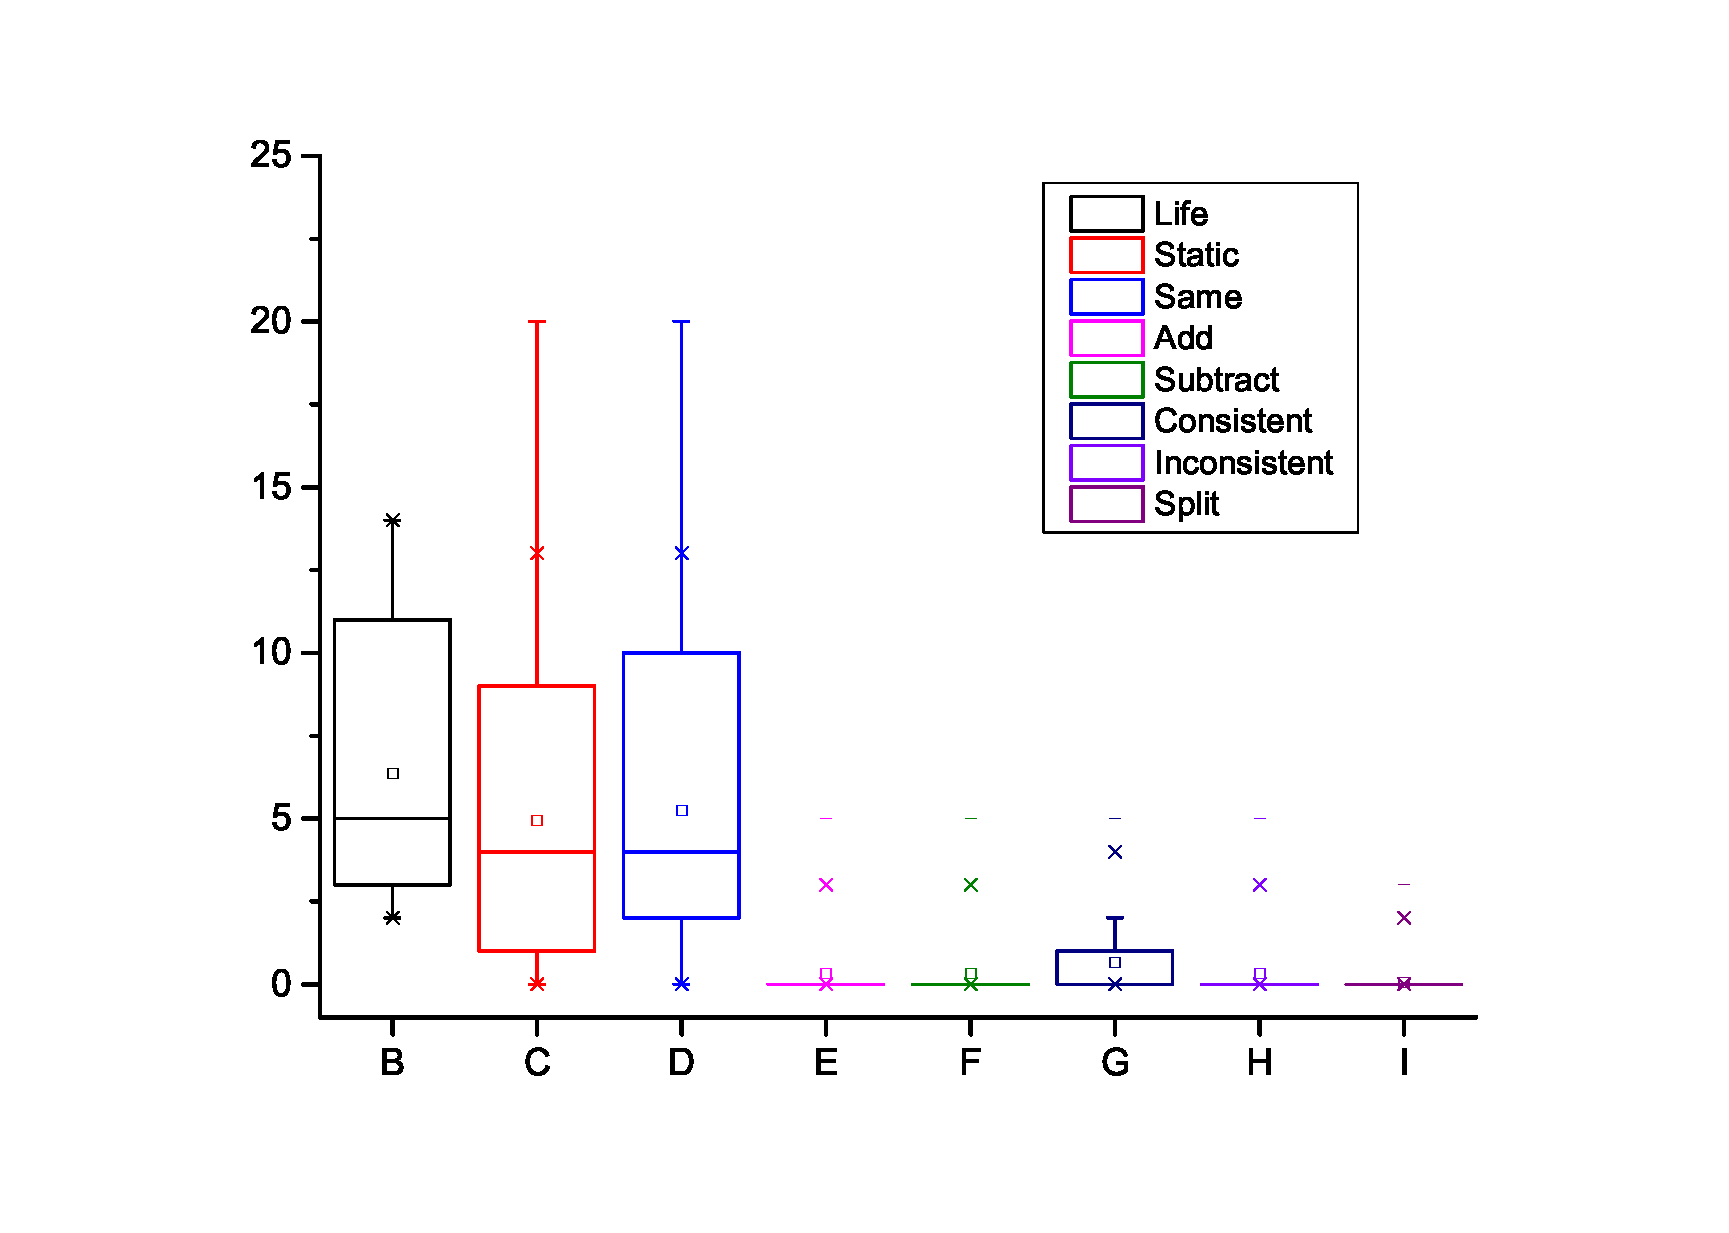
\includegraphics[width=3.3in]{Fig3a.eps} }
    \end{subfigure}
    \begin{subfigure}[jEdit]
    { {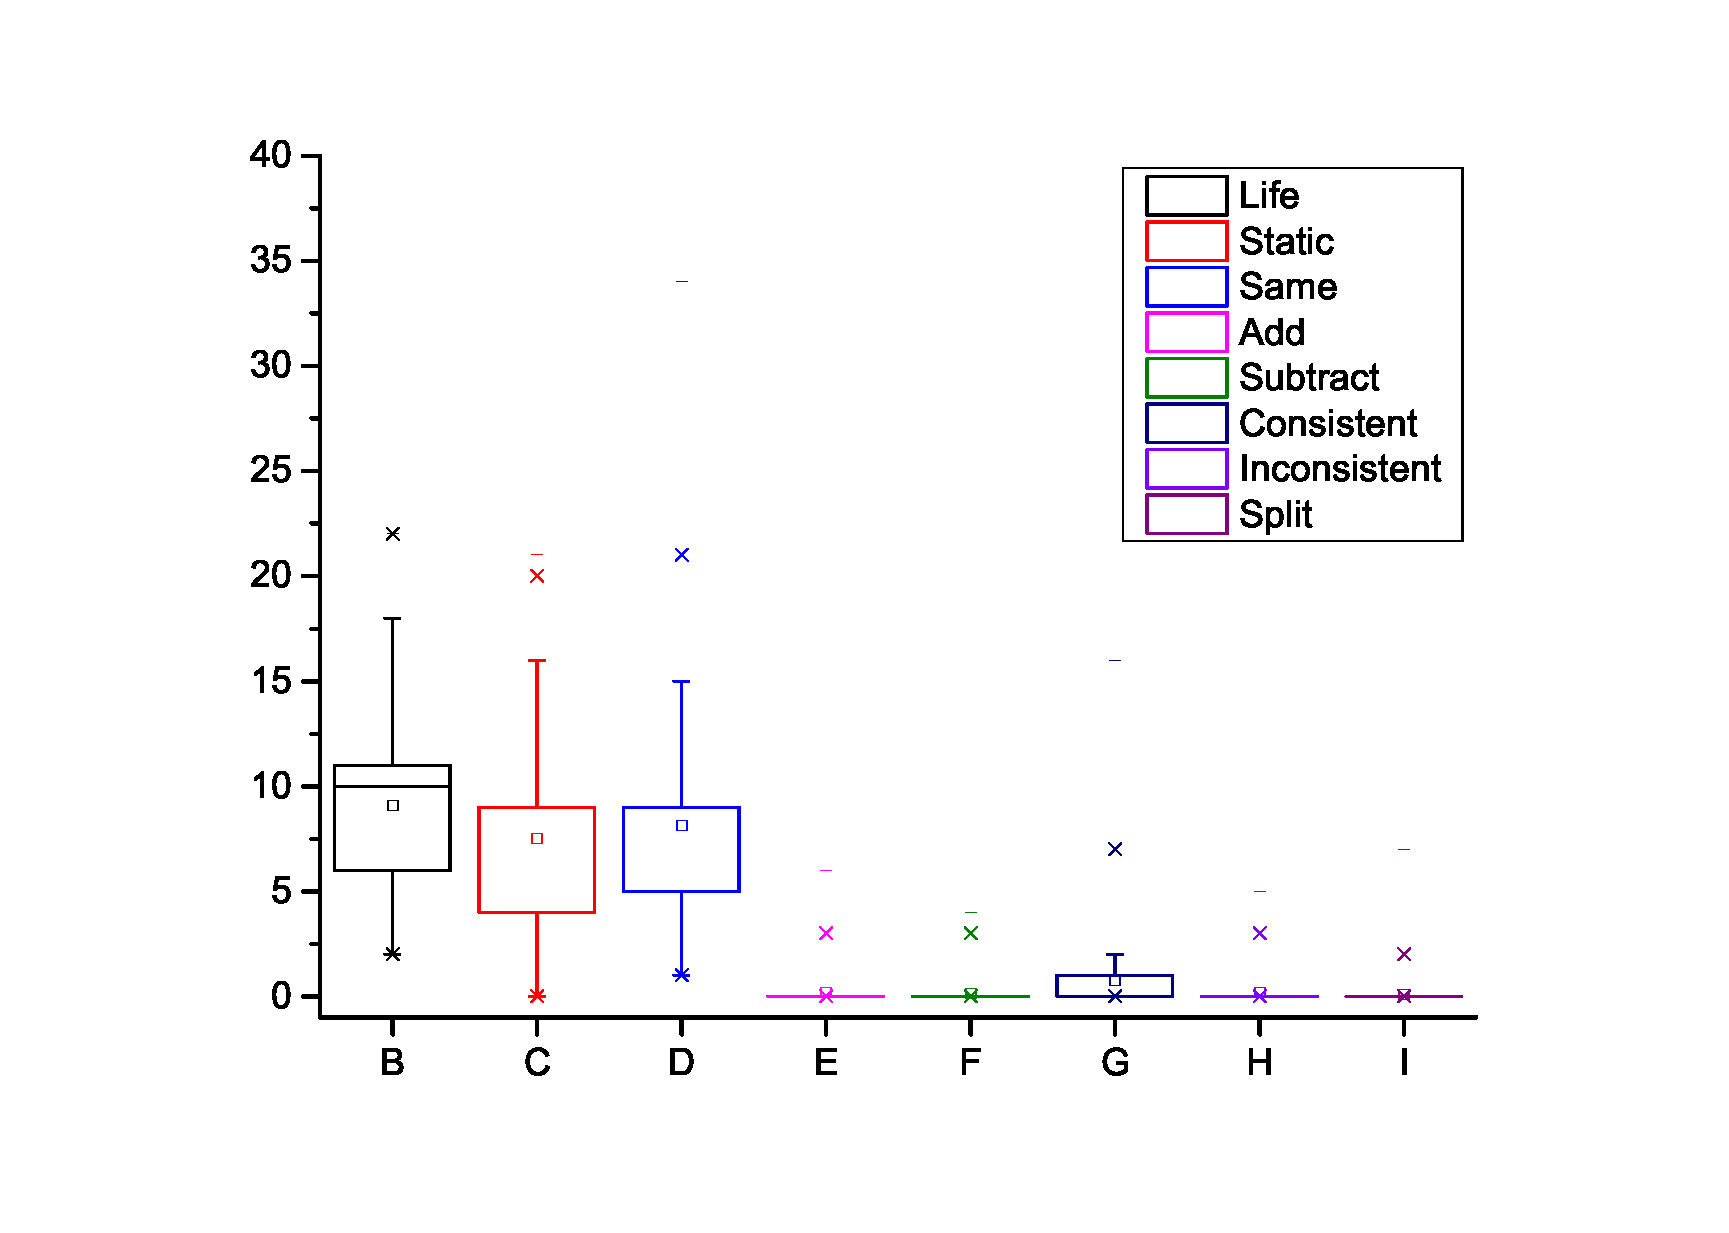
\includegraphics[width=3.3in]{Fig3b.eps} } }
    \end{subfigure}
    \centerline{\footnotesize\begin{tabular}{c} Fig.\ 3.\ Clone Genealogy Statistics Results
\end{tabular}}
\end{figure*}

Tables 8 and 9 depict the results of clone group clustering. Here, Cluster 1 has the largest number of clone groups (71\% in {\em ArgoUML}, 79\% in {\em jEdit}), and these clone groups are relatively stable (have stable clone pattern, do not have dynamic clone pattern), and have relatively longer lives. Therefore, {\em most of clone groups are very stable, which also have a relatively longer life (about 5 versions both in the two software)}. Most of the {\em inconsistent change pattern} appear in Cluster 0, which take up only a small percentage (4\% in {\em ArgoUML}, only 1\% in {\em jEdit}). Therefore, {\em inconsistent change does not frequently occur in clone group}. Meanwhile, {\em consistent change pattern} occurs only in Cluster 2, which also has a relatively longer life --- but shorter than Cluster 0. Both Cluster 0\&2 are dynamic clone groups because they both have the dynamic clone pattern. We conclude that, {\em dynamic clone pattern occurs in longer life clone group, and their number is very small}.  

If we check the absolute number of groups in Cluster 0\&2, we see that the number of clone group having consistent changes (Cluster 2) is bigger than those having inconsistent changes (Cluster 0).  This means {\em consistent change is much easily occurring than inconsistent change}. Thus, we suggest that: {\em Developers should consider the possibility of performing consistent change when they detect that a clone fragment has undergone some change}.  

Cluster 3 shows that there is quite a proportion of clone groups having extremely short life (which just appear in systems), which have no clone pattern. This means that {\em we need not consider the effect of changes in clone group at the initial version of clone group creation}.   

In summary, clone groups are generally very stable throughout evolution. Dynamic clone pattern may happen after the clone groups have been in existence for a while, but only for a small proportion of them. When developers change a particular clone fragment, it is advisable for them to also consider the change in the context of clone group and determine if consistent change need to be made across the entire group.

\leftline{{\bf5.3 \ Clone Genealogy Experiment}}

In studying the characteristics of clone genealogy, which offers a global perspective, we first compute the number of clone pattern occurring in its entire life for each of clone genealogies, and then perform clustering on these clone genealogies using their metrics. 

We first compute the statistics for each of the metrics (including genealogy life and clone patterns) in all the clone genealogies. The results are plotted in Fig.3 using ``Box-and-Whisker'' diagrams.  The first (extreme left) box shows the statistics about genealogy lives. For the rest of the boxes in the plot, each of them represents the statistics for each clone pattern. 

{
\begin{table*}[!htb]
\tabcolsep=2.5pt 
\scriptsize
\begin{center}
\begin{tabular}{|c|c|c|c|c|c|c|c|c|c|c|}
\multicolumn{11}{c}{\bf Table 10.\  Clone Genealogy Clustering Results of ArgoUML }\\ \hline
&Death&&Genealogy Life&	Static&	Same&	Add	&Subtract&	Consistent&	Inconsistent&	Split\\ \hline
Cluster0&\multirow{3}{*}{5}&Mean	&11.85366	&9.79268	&10.45122	&2.23171&	2.23171&	3.06098&	2.29268&	0.39024\\ \cline{3-11}
82&&Standard Deviation	&1.81979	&2.98861&	3.04758&	1.04585&	1.08068	&0.85125&1.07138&	0.84263\\ \cline{3-11}
(8\%)&&Median	&11&	10&	10&	2&	2&	3&	2	&0\\ \hline
Cluster1&\multirow{3}{*}{39}&Mean	&10.19221	&8.83117	&9.0961	&0.17143	&0.12208	&0.44416	&0.12208	&0.00519\\ \cline{3-11}
385&&Standard Deviation&	1.67998	&1.67552	&1.70282	&0.39754&	0.3278	&0.64761&	0.3278	&0.10193\\ \cline{3-11}
(37\%)&&Median	&11	&9	&10	&0&	0&	0&	0	&0\\ \hline
Cluster2&\multirow{3}{*}{188}&Mean	&3.29412	&1.2549	&2	&0.47059	&0.46078	&1.2598	&0.46078	&0.0098\\ \cline{3-11}
204&&Standard Deviation	&1.22847	&1.35506	&1.32427	&0.63875	&0.63822	&0.43961	&0.63822	&0.14003\\ \cline{3-11}
(20\%)&&Median	&3&	1&	2&	0&	0&	1&	0&	0\\ \hline
Cluster3&\multirow{3}{*}{348}&Mean	&2.79452	&1.79452	&1.79452	&0	&0	&0	&0	&0\\ \cline{3-11}
365&&Standard Deviation	&1.0813	&1.0813	&1.0813	&0	&0	&0	&0	&0\\ \cline{3-11}
(35\%)&&Median	&3	&2	&2	&0	&0	&0&	0&	0\\ \hline
All&\multirow{3}{*}{579}&Mean	&6.35907	&4.93629	&5.23359	&0.33301	&0.31274	&0.65541	&0.31757	&0.03475\\ \cline{3-11}
1036&&Standard Deviation	&4.02533	&4.0219	&4.06154	&0.74995	&0.74514	&0.97405	&0.75663	&0.27231\\ \cline{3-11}
(100\%)&&Median&	5&	4&	4&	0&	0&	0&	0&	0\\ \hline
\end{tabular}
\end{center}
\end{table*}
}
{
\begin{table*}[!htb]
\tabcolsep=2.5pt 
\scriptsize
\begin{center}
\begin{tabular}{|c|c|c|c|c|c|c|c|c|c|c|}
\multicolumn{11}{c}{\bf Table 11.\  Clone Genealogy Clustering Results of jEdit }\\ \hline
&Death&&Genealogy Life&	Static&	Same&	Add	&Subtract&	Consistent&	Inconsistent&	Split\\ \hline
Cluster0&\multirow{3}{*}{3}&Mean	&19	&15.8	&19.2	&3	&2.3&	6	&2.7&	1.1\\ \cline{3-11}
10&&Standard Deviation	&4.83046	&4.56557&	6.42564	&1.33333&	0.94868&	4.57044&	1.41814	&2.23358\\ \cline{3-11}
(4\%)&&Median	&22&	17&	19&	3&	2	&4.5	&2.5&	0\\ \hline
Cluster1&\multirow{3}{*}{35}&Mean	&10.95205&	9.44521&	9.93836&	0.07534	&0.07534	&0.58904&	0.08219&	0.0411\\ \cline{3-11}
146&&Standard Deviation&2.35572	&2.16566&2.35832	&0.26485	&0.31262&	1.07428&	0.34254&	0.28471\\ \cline{3-11}
(62\%)&&Median&	10&	9&	9	&0&	0	&0	&0&	0\\ \hline
Cluster2&\multirow{3}{*}{24}&Mean	&6.57143&	4.75&	5.60714&	0.07143&	0.07143&	0.85714&	0.07143&	0.07143\\ \cline{3-11}
28&&Standard Deviation	&1.16837&	1.14261	&1.22744	&0.26227&0.26227	&0.97046	&0.26227	&0.37796\\ \cline{3-11}
(12\%)&&Median	&7	&5	&6&	0	&0	&1&	0&	0\\ \hline
Cluster3&\multirow{3}{*}{48}&Mean	&3.33962&	2.13208&	2.30189&	0.03774&	0	&0.20755&	0	&0\\ \cline{3-11}
53&&Standard Deviation&	0.73231	&0.92065	&0.72284&	0.19238&	0&	0.45398	&0	&0\\ \cline{3-11}
(22\%)&&Median	&3&	2&	2	&0&	0&	0	&0&	0\\ \hline
All&\multirow{3}{*}{110}&Mean	&9.07173	&7.52321&	8.1097	&0.18987&	0.1519&	0.76371	&0.173&	0.08017\\ \cline{3-11}
237&&Standard Deviation	&4.36559&	4.07926	&4.56922	&0.6903&	0.55438&	1.70588	&0.66354	&0.55033\\ \cline{3-11}
(100\%)&&Median	&10	&9	&9	&0	&0	&0	&0	&0\\ \hline
\end{tabular}
\end{center}
\end{table*}
}

We can see that clone genealogy exist in the systems for a reasonably long period of time (i.e.  {\em mean value of life} is 5 versions for {\em ArgoUML} within the entire 14 versions, and 10 versions for {\em jEdit} with the entire 22 versions), and only a small part of clone genealogy exists for extremely short (less than 3 versions) or extremely long (more than 10 versions) life. We also see that the number of {\em stable clone pattern} is much higher than the number of {\em dynamic clone pattern}. For {\em dynamic clone pattern}, their numbers are extremely few, expect for {\em consistent change pattern}. {\em It means that clone genealogy is very stable during the life of clone evolution.} Specially, the number of ``consistent change'' outnumbers that of ``inconsistent change''. This implies that {\em it is worth paying attention to determine if a clone change should be propagated to other clones in the same clone group}. 

We use X-means clustering to mine more information from clone genealogy between the {\em life} and {\em clone patterns}. In Tables 10 and 11, we define a special variable called {\em Death} which reports the number of clone genealogies which have ended their lives before reaching the last version collected in the experiment. By knowing that a genealogy contributes to a count in {\em Death}, we know that the data we obtained in the experiment for clone genealogy is ``complete''; the genealogy does not get terminated prematurely by our selection of software versions.  The second column in these tables thus shows the number of the death clone genealogy. 

According to clustering results, all clone genealogies can be clustered into four clusters, as shown as in the tables. From Fig. 3/Tables 10 \& 11, it is clear that {\em there is a strongly positive correlation between the genealogy life and stable pattern}. We informally define a genealogy to be {\em stable} if it has a high percentage of {\em stable clone pattern}% (which are represented by high numbers of ``static'' and ``same'' metrics)
; otherwise, we say that a genealogy is {\em dynamic}% (that is, it has a relatively large collection of ``add'', ``subtract'', ``consisten'', ``inconsistent'' and ``split'' clone patterns)
. From the tables, we can see that: {\em most of the clone genealogies are stable (Cluster 1,2,3)}. On the other hand, there are much fewer dynamic genealogies (in Cluster 0, having long lives, and most of them are still alive in the systems). It tells us {\em dynamic clone pattern -- especially consistent/inconsistent change -- usually occur in the longer life clone genealogy. Moreover, the number of dynamic genealogy is small}. This suggests that developers should take some measures on {\em dynamic genealogy} because inconsistent change may lead to software defects. For Cluster 3 (both in tables 10,11), the respective clone genealogies have relatively shorter lives, and most of them are already dead. These clone genealogies are extremely stable because the absence of inconsistent pattern. {\em Therefore, it can be concluded that the clones in short life clone genealogies are more stable than the older ones. It can give us a hint that, developers may not need to keep their eyes on newly created (shorter life) clone genealogy. But, they should pay attention to them, when they evolve together with the software.}

In summary, clone genealogies are mostly stable throughout evolution. The shorter-life genealogies are especially stable. {\em Dynamic change pattern} usually occurs among longer-life genealogies, even though the appearance remains sparse. Among them, consistent changes appear more frequently than inconsistent ones. With that, we suggest that developers should pay attention to longer-life clone genealogies, and consider the possibility of allowing consistent change to a clone group when one clone fragment in the group is about to undergo changes.


%\begin{center}{\large\bf 6. Discussion}\end{center}
\begin{center}{\large\bf 6. Discussion}\end{center}

Our method depends on NiCad and clone mapping algorithm to build clone genealogy. We use NiCad to detect clones, the results of which are then used for mapping the clones so as to build clone genealogy. A more refined clone detection tool and a more accurate clone mapping algorithm may possibly improve the quality of the subsequent phases. Note that our approach strongly depends on the availability of clone metrics. We use a set of metrics to represent clone fragment, clone group, clone genealogy. While these metrics have served us well, we would like to expand the collection of metrics in the future, as new interesting metrics can hint on possibly new relationship between clones and their evolution. 

In the future, we can also conduct more experiments on different softwares with more clone metrics. We believe that we have presented some more meaningful conclusions to help clone analysis and clone maintenance. We can also do some further work on clone characteristics. We believe that clone characteristics should be used in clone analysis during system maintenance. For instance, we can identify some special clone from softwares, and we intend to link this to clone harmfulness. 



%\begin{center}{\large\bf 7.\ Conclusion}\end{center}
\begin{center}{\large\bf 7.\ Conclusion}\end{center}

In this paper, we propose an approach to analyze clone evolutionary characteristics through machine learning method from clones and their evolution. Specifically, we have demonstrated the usefulness of clustering (via X-means algorithm) the clone entities by taking into consideration the life times of clone entities. %The contributions of our paper include: (1) we propose a framework to analyze the clone characteristics for multi-version softwares. (2) We extract a class of relevant clone metrics to characterize clone fragment, clone group and clone genealogy. We provide three different perspectives about clone evolution, so that conclusions can be drawn from all aspects of clone evolution, from individual clone perspective to global-based genealogy perspective. (3) We conduct a case study on two softwares: {\em ArgoUML} and {\em jEdit} to explore the clone evolutionary characteristics. 
Our case study shows that clones are in general very stable during their evolution, and clones usually do not undergo changes at the infancy stage of evolution. Developers should therefore pay more attention to (more matured) clones that have existed in a genealogy after several evolutions (aka., in longer life clone genealogy). We also suggest that developers should consider the possibility of making consistent changes across the entire clone group when one of the constituent clone fragments has undergo change. 

We believe that these characteristics can help developers to understand clones better, and can also provide some guidance to maintain and manage clones in software development. In future, we intend to improve our analysis on clone group and clone genecology by incorporating more metrics. The conclusion drawn about the relationships on clone group and genealogy can be viewed as the features of clone evolution. These features may be helpful for clone management.


%\begin{center}{\large\bf  Acknowlwdgment}\end{center}
%This work is supported by a National Natural Science Foundation of China under Grant %No.61173021.

\RE

\footnotesize\rm

\REF{[1]} Roy C K, Cordy J R. A survey on software clone detection research[R]. Technical Report 541, Queen's University at Kingston, 2007. 
\REF{[2]} Koschke R. Survey of research on software clones[M]. Internat. Begegnungs-und Forschungszentrum f\"{u}r Informatik, 2007.
\REF{[3]} Kim M, Sazawal V, Notkin D, et al. An empirical study of code clone genealogies[C]//ACM SIGSOFT Software Engineering Notes. ACM, 2005, 30(5): 187-196.
\REF{[4]} Kapser C, Godfrey M W. " Cloning considered harmful" considered harmful[C]//Reverse Engineering, 2006. WCRE'06. 13th Working Conference on. IEEE, 2006: 19-28.
\REF{[5]} Inoue K, Higo Y, Yoshida N, et al. Experience of finding inconsistently-changed bugs in code clones of mobile software[C]//Proceedings of the 6th International Workshop on Software Clones. IEEE Press, 2012: 94-95.
\REF{[6]} Krinke J. Is cloned code more stable than non-cloned code?[C]//Source Code Analysis and Manipulation, 2008 Eighth IEEE International Working Conference on. IEEE, 2008: 57-66.
\REF{[7]} Roy C K, Zibran M F, Koschke R. The vision of software clone management: Past, present, and future (keynote paper)[C]//Software Maintenance, Reengineering and Reverse Engineering (CSMR-WCRE), 2014 Software Evolution Week-IEEE Conference on. IEEE, 2014: 18-33.
\REF{[8]} Koschke R, Baxter I, Conradt M, et al. Software clone management towards industrial application[C]//Dagstuhl Seminar: Software Clone Management Towards Industrial Application. 2012.
\REF{[9]} Roy C K, Cordy J R. NICAD: Accurate detection of near-miss intentional clones using flexible pretty-printing and code normalization[C]//Program Comprehension, 2008. ICPC 2008. The 16th IEEE International Conference on. IEEE, 2008: 172-181.
\REF{[10]} Kamiya T, Kusumoto S, Inoue K. CCFinder: a multilinguistic token-based code clone detection system for large scale source code[J]. Software Engineering, IEEE Transactions on, 2002, 28(7): 654-670.
\REF{[11]} Tairas R A. Representation, analysis, and refactoring techniques to support code clone maintenance[D]. The University of Alabama at Birmingham, 2010.
\REF{[12]} Nguyen H A, Nguyen T T, Pham N H, et al. Clone management for evolving software[J]. Software Engineering, IEEE Transactions on, 2012, 38(5): 1008-1026.
\REF{[13]} Bettenburg N, Shang W, Ibrahim W, et al. An empirical study on inconsistent changes to code clones at release level[C]//Reverse Engineering, 2009. WCRE'09. 16th Working Conference on. IEEE, 2009: 85-94.
\REF{[14]} Wang X, Dang Y, Zhang L, et al. Can I clone this piece of code here?[C]//Proceedings of the 27th IEEE/ACM International Conference on Automated Software Engineering. ACM, 2012: 170-179.
\REF{[15]} Yang J, Hotta K, Higo Y, et al. Classification model for code clones based on machine learning[J]. Empirical Software Engineering, 2014: 1-31.
\REF{[16]} Qu W, Jia Y, Jiang M. Pattern mining of cloned codes in software systems[J]. Information Sciences, 2014, 259: 544-554.
\REF{[17]} Rattan D, Bhatia R, Singh M. Software clone detection: A systematic review[J]. Information and Software Technology, 2013, 55(7): 1165-1199
\REF{[18]} Duala-Ekoko E, Robillard M P. Clonetracker: tool support for code clone management[C]//Proceedings of the 30th international conference on Software engineering. ACM, 2008: 843-846.
\REF{[19]} Duala-Ekoko E, Robillard M P. Clone region descriptors: Representing and tracking duplication in source code[J]. ACM Transactions on Software Engineering and Methodology (TOSEM), 2010, 20(1): 3.
\REF{[20]} Bakota T. Tracking the evolution of code clones[M]//SOFSEM 2011: Theory and Practice of Computer Science. Springer Berlin Heidelberg, 2011: 86-98.
\REF{[21]} Bakota T, Ferenc R, Gyimothy T. Clone smells in software evolution[C]//Software Maintenance, 2007. ICSM 2007. IEEE International Conference on. IEEE, 2007: 24-33.. 
\REF{[22]} Harder J, Göde N. Cloned code: stable code[J]. Journal of Software: Evolution and Process, 2013, 25(10): 1063-1088. 
\REF{[23]} Rahman F, Bird C, Devanbu P. Clones: What is that smell?[J]. Empirical Software Engineering, 2012, 17(4-5): 503-530.
\REF{[24]} Lin Y, Xing Z, Xue Y, et al. Detecting differences across multiple instances of code clones[C]//Proceedings of the 36th International Conference on Software Engineering. ACM, 2014: 164-174.
\REF{[25]}Mark H, Eibe F, Geoffrey Holmes, Bernhard Pfahringer, Peter Reutemann, Ian H. Witten (2009); The WEKA Data Mining Software: An Update; SIGKDD Explorations, Volume 11, Issue 1.
\REF{[26]} Pelleg D, Moore A W. X-means: Extending K-means with Efficient Estimation of the Number of Clusters[C]//ICML. 2000, 1.
%\REF{[27]} Meng Ci, Xiao-hong Su, Tian-tian Wang, et al. A New Clone Group Mapping Algorithm for Extracting Clone Genealogy on Multi-version Software[C]//Instrumentation, Measurement, Computer, Communication and Control (IMCCC), 2013 Third International Conference on. IEEE, 2013: 848-853. 

\end{multicols} %双栏结束
\end{document}}
